\documentclass[12pt]{article}
\usepackage[margin=1in]{geometry} 
\usepackage{amsmath,amsthm,amssymb,amsfonts}
\usepackage{graphicx,fancyhdr,algorithm,algorithmic}
\usepackage[space]{grffile}
\usepackage{titlesec}
\usepackage{multicol}
\usepackage{enumitem} 
\usepackage{tikz}
\usepackage{tikz-qtree}
\usetikzlibrary{arrows,automata}


\cfoot{\thepage}
\renewcommand{\headrulewidth}{0.4pt}
\renewcommand{\headwidth}{\textwidth}
\renewcommand{\footrulewidth}{0.4pt}


\theoremstyle{definition}
\newtheorem{problem}{Problem}
\newtheorem{claim}{Claim}
\newtheorem{definition}{Definition}
\newtheorem{theorem}{Theorem}
\newtheorem{lemma}{Lemma}
\newtheorem{observation}{Observation}
\newtheorem{question}{Problem}

\newenvironment{solution}{\bigskip\noindent{\it Solution.}  \ignorespaces}{\hfill\qed}

\usepackage{hyperref}
\hypersetup{
    colorlinks=true,
    linkcolor=blue,
    filecolor=magenta,      
    urlcolor=cyan,
}
\urlstyle{same}
\PassOptionsToPackage{hyphens}{url}
\newcommand{\homework}[6]{
   \pagestyle{myheadings}
   \thispagestyle{plain}
   \newpage
   \setcounter{page}{1}
   \noindent
   \begin{center}
   \framebox{
      \vbox{\vspace{2mm}
    \hbox to 6.28in { {\bf CS256:~Algorithm Design and Analysis \hfill #1} }
       \vspace{6mm}
       \hbox to 6.28in { {\Large \hfill #2 \normalsize{(#3)}  \hfill} }
       \vspace{6mm}
     \hbox to 6.28in { {\it Instructor: #4 \hfill  Solution template: #5} }
   }
   }
   \end{center}
   \markboth{#1}{#1}
   \vspace*{4mm}
}

\begin{document}
\homework{Spring 2021}{Assignment 4}{due 03/24/2021 }{Shikha Singh}{\href{https://www.overleaf.com/read/zrybwmzrjrhz}{\em Overleaf}, \href{https://williams-cs.github.io/cs256-s21-www/assignments/Assignment_4.tex}{\em .tex}}




\begin{question}
  Use any of the methods discussed in class (unfolding recurrences, recursion trees, master theorem, guess and check etc.) to solve each of the following recurrences. Give as tight a Big Oh bound as possible. You must justify (at a high level) your answer in each case---e.g., if using the recursion-tree method, draw the first few levels of the tree and describe which of the three categories does the recurrence lie in, and why that leads to the time bound. You do not need to verify by induction (unless you are using the guess and check method in which case you do need a proof). You may use a package to draw figures or attach a scan of a neatly hand-drawn figure.  The first part is solved to guide your approach.


\begin{enumerate}[label = (\alph*)]
    \item\label{1a} $T(n) = 2T(n/2) + n^2$
    
    \begin{solution}
     The recursion tree for this recurrence is given in Figure~\ref{rectree}. Notice that the cost at each level is decreasing by at least a constant factor.
     The total cost at the root is $n^2$, one level down is $n^2/2$, and two levels down is $n^4/4$.
     In particular we get the following decaying geometric series $T(n) = n^2 (1 + 1/2 + 1/4 + \ldots) = \Theta(n^2)$.
     This falls into the first category of the recursion-tree method and the cost is dominant at the root, that is, $T(n) = O(n^2)$.
    \begin{figure}[h]
    \vspace{-10pt} 
    \centering
    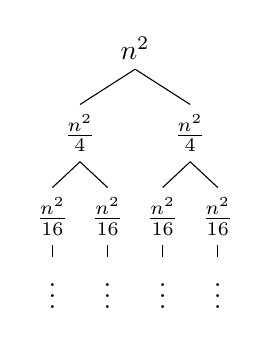
\begin{tikzpicture}
      %this package is useful for quickly making nice-looking trees
      %whitespace is unimportant: [ makes a new tree node; ] completes the node
    \Tree [.$n^2$ 
            [.${\frac{n^2}{4}}$ 
              [.${\frac{n^2}{16}}$ $\vdots$ ] 
              [.${\frac{n^2}{16}}$ $\vdots$ ] 
            ] 
            [.${\frac{n^2}{4}}$ 
              [.${\frac{n^2}{16}}$ $\vdots$ ] 
              [.${\frac{n^2}{16}}$ $\vdots$ ] 
            ] 
          ]
    \end{tikzpicture}\caption{Recursion Tree for Problem~1 \ref{1a}}\label{rectree}
    \end{figure}   
    \vspace{-10pt} 
    \end{solution}

     
    \item $T(n) = 2T(n/4) + \sqrt{n}$
    \item $T(n) = 3T(n/3) + O(n^2)$
    \item $T(n) = 2T(n/2) + n \log n$ 
\end{enumerate}
\end{question}

\begin{solution}
\begin{enumerate}

\item[(b)]

\item[(c)]

\item[(d)]
\end{enumerate}
\end{solution}


\newpage
\begin{question}\label{majority}
  You're running an internet poll on a popular website.  Each user on the website is only allowed to vote once in the poll.  Of course, there's an obvious problem: some people have multiple user accounts on the website.

  You want to rule out the worst-case scenario: is there a single person who controls the \emph{majority} of the user accounts on the site?  

  You receive an array of usernames $U[1\ldots n]$.  You want to determine if a single person controls $> \lceil n/2 \rceil$ of the usernames.  You don't know which person controls a given username; however you have access to two subroutines:
  \begin{itemize}
    \item \textsc{samePerson($i$,$j$)} takes two integers $i$ and $j$ and returns whether or not $U[i]$ and $U[j]$ are controlled by the same person, in $O(1)$ time.\footnote{Let's say this runs some simple analytics on the metadata we've stored for the two users.}
    \item \textsc{countOccurrences($i$,$\ell$,$r$)} returns the number of usernames in $U[\ell, \ell+1,\ldots, r]$ controlled by the same person that controls $U[i]$, in $O(r - \ell + 1)$ time.\footnote{This is easy to implement---just call \textsc{samePerson($i$,$j$)} for $j = \ell, \ldots, r$.  Having this as a subroutine, rather than a whole loop, may make your algorithm simpler.}
  \end{itemize}

  Notice that we can run \textsc{countOccurrences($i$,$1$,$n$)} for all $i = 1,\ldots n$ and learn exactly how many accounts each person controls, in $O(n^2)$ time.

  Instead, you are to design an algorithm that determines if a single person controls $> \lceil n/2 \rceil$ of the usernames, in $O(n\log n)$ time.
To avoid edge cases, assume $n$ has a nice form, e.g., a power of $2$.
You must
prove that your algorithm is correct (under the assumption that \textsc{samePerson} and \textsc{countOccurrences} are correct). 
State and solve the recurrence for the running time of your algorithm.
\end{question}
\begin{solution}
\end{solution}


\newpage
\begin{question} 
Suppose we are given two sorted arrays $A[1 \ldots n]$ and $B[1 \ldots n]$. 
Assume that the arrays do not contain duplicate
elements. Describe an algorithm to find the median of $A \cup B$ in $O(\log n)$ time.
The median of sorted array $A$ of size $n$ is the middle element (at index $(n+1)/2$) if $n$ is odd; and is
the average of the two middle elements (at indices $n/2$ and $(n+1)/2$)
if $n$ is even.  Remember to {justify the correctness of your algorithm} 
and state and solve its running time recurrence.
\end{question}
\begin{solution}
\end{solution}


\newpage
\begin{question}
Consider the following funky recursive sorting algorithm called \textsc{funky-sort}.

\vspace{10pt}
\noindent
\textsc{funky-sort}$(A[1, \ldots, n)$:\\
\hspace*{5mm} if $n = 2$ and $A[1] > A[2]$:\\
\hspace*{5mm} \hspace*{6mm}swap $A[1] \leftrightarrow A[2]$\\
\hspace*{5mm} else if $n >2$:\\
\hspace*{5mm} \hspace*{6mm}$m = \lceil 2n/ 3 \rceil$\\
\hspace*{5mm} \hspace*{6mm}\textsc{funky-sort}$(A[1, \ldots, m])$\\
\hspace*{5mm} \hspace*{6mm}\textsc{funky-sort}$(A[n-m+1, \ldots, n])$\\
\hspace*{5mm} \hspace*{6mm}\textsc{funky-sort}$(A[1, \ldots, m])$

\begin{enumerate}[label = (\alph*), noitemsep]
    \item Does \textsc{funky-sort} actually sort the array?  Prove its correctness if you think it does, otherwise give a counterexample.
    \item State and solve the recurrence for the running time of \textsc{funky-sort}.
\end{enumerate}
\end{question}
\begin{solution}
\end{solution}

\newpage
\begin{question}({\bf Extra Credit (7 pts)})
  The company UPS has noticed that left turns are extremely costly---trucks must idle for a long time looking for an opportunity to turn left.  In fact, when determining routes for drivers, they eliminate almost all left turns from the route.  This saves the company over 300 million dollars per year.  See this url for one article on this policy: \url{https://www.cnn.com/2017/02/16/world/ups-trucks-no-left-turns/index.html}

  Let's apply the same logic to shortest path.  Define two edges along a path $(v_1,v_2), (v_2, v_3)$ to be a \textbf{left turn} if:
  \begin{itemize}[topsep=0pt,noitemsep]
    \item $v_3$ is immediately before $v_1$ in the adjacency list of $v_2$, or 
    \item $v_3$ is the last vertex in the adjacency list of $v_2$ and $v_1$ is the first.
  \end{itemize}

  Given an undirected graph $G$ where all edges have a positive weight, and two nodes $s$ and $t$, let the \textbf{UPS shortest path} be the shortest path from $s$ to $t$ that does not take a left turn.

  Design an efficient algorithm to compute the {UPS shortest path}.  Analyze its running time and briefly explain its correctness.
\end{question}
\begin{solution}
\end{solution}

\newpage
\subsection*{Acknowledgement}
This is where you cite your sources and collaborators.


\end{document}

